\documentclass[hyperpdf, nobind]{hepthesis}
%% For Cambridge hard-bound version (must be one-sided)
%\documentclass[hyperpdf,oneside]{hepthesis}

\usepackage[T2A]{fontenc}
\usepackage[utf8]{inputenc}
\usepackage[russian]{babel}
\usepackage{amsfonts}
\usepackage{amsmath}
\usepackage{graphicx}
%\graphicspath{/images}
\usepackage{float}
\usepackage{caption}
\usepackage{subcaption}

%% Load special font packages here if you wish
%\usepackage{lmodern}
%\usepackage{mathpazo}
%\usepackage{euler}
\usepackage{iwona}

\allowdisplaybreaks


\title{
\textcyrillic{Механизмы сосуществования стационарных биологических сообществ в пространствах разных размерностей}}
\author{Антон Сергеевич Савостьянов}


\begin{document}


\begin{frontmatter}
  %% Title
\titlepage[$\cdot$ \\ Руководитель: Никитин Алексей Антонович, \\ доцент, к.ф.-м.н]{%
Выпускная Квалификационная Работа \\
студента бакалавриата Факультета Компьютерных Наук \\
НИУ "Высшая Школа Экономики"}

%% Abstract
\begin{abstract}%[\smaller \thetitle\\ \vspace*{1cm} \smaller {\theauthor}]
  %\thispagestyle{empty}
  \LHCb is a \bphysics detector experiment which will take data at
  the \unit{14}{\TeV} \LHC accelerator at \CERN from 2007 onward\dots
\end{abstract}


%% Declaration
\begin{declaration}
  This dissertation is the result of my own work, except where explicit
  reference is made to the work of others, and has not been submitted
  for another qualification to this or any other university. This
  dissertation does not exceed the word limit for the respective Degree
  Committee.
  \vspace*{1cm}
  \begin{flushright}
    Andy Buckley
  \end{flushright}
\end{declaration}


%% Acknowledgements
\begin{acknowledgements}
  Of the many people who deserve thanks, some are particularly prominent,
  such as my supervisor\dots
\end{acknowledgements}


%% Preface
\begin{preface}
  This thesis describes my research on various aspects of the \LHCb
  particle physics program, centred around the \LHCb detector and \LHC
  accelerator at \CERN in Geneva.

 % \noindent
%  For this example, I'll just mention \ChapterRef{chap:SomeStuff}
%  and \ChapterRef{chap:MoreStuff}.
\end{preface}

%% ToC
\tableofcontents


%% Strictly optional!
\frontquote{%
  Writing in English is the most ingenious torture\\
  ever devised for sins committed in previous lives.}%
  {James Joyce}
%% I don't want a page number on the following blank page either.
\thispagestyle{empty}

\end{frontmatter}

\begin{mainmatter}
  \chapter{Введение}
\label{chap:Intro}

%% Restart the numbering to make sure that this is definitely page #1!
\pagenumbering{arabic}

%% Note that the citations in this chapter use the journal and
%% arXiv keys: I used the SLAC-SPIRES online BibTeX retriever
%% to build my bibliography. There are also quite a few non-standard
%% macros, which come from my personal collection. You can have them
%% if you want, or I might get round to properly releasing them at
%% some point myself.

%\chapterquote{Laws were made to be broken.}%
%{Christopher North, 1785--1854}%: Blackwood's Magazine May 1830

% Антон Савостьянов, [24.01.17 15:31]
%Ячейки бенара

%Антон Савостьянов, [24.01.17 15:32]
%Лизеганга

%Антон Савостьянов, [24.01.17 15:34]
%Белоусова Жаботинского

%Антон Савостьянов, [24.01.17 15:41]
%Dictostelium discoideum

%Антон Савостьянов, [24.01.17 15:51]
%E. Coli

В 1916 году в \cite{einstein} Альберт Эйнштейн (Albert Einstein) предложил концепцию вынужденного излучения (stimulated emission) --- возникновения колебаний возбужденных электронов, индуцированного существующей световой волной: согласно предложенной теории, данный процесс порождает набор разнофазовых эквиамплитудных волн, \emph{конкурентная самоорганизация} которых в стационарном положении образует равномерно колеблющуюся волну, явление, также известное как \emph{лазерное излучение} \cite{steen}. 

Самоорганизация мультиагентных естественных процессов подробно изучалась в случае химических систем: в 1896 Рафаэелем Лизегангом (Raphael E. Liesegang)  был рассмотрен процесс формирования структур, являющихся следствием выпадения в осадок вещества, получившегося в результате химической реакции, (кольца Лизеганга) \cite{leis}. Другими широкоизвестными феноменами являются реакция Белоусова-Жаботинского \cite{belousov} и ячейки Релея-Бенара \cite{benard}.

  \chapter{Модель самоструктурирующихся сообществ Ульфа Дикмана}

В данной части настоящей работы вводится модель самоструктурирующихся в пространстве сообществ, предложенная Ульфом Дикманом (Ulf Dieckmann)  и Ричардом Лоу (Richard Law) в \cite{law_dieckmann_2000,law_2003}; вводится предлагаемое пространство состояний системы, описываемой набором статистик, отвечающих за естественные степени свободы популяции; описывается пространство параметров системы и динамика предложенный статистик относительно данного пространства параметров; обсуждается техника аппроксимаций (замыканий) набора статистик высшего порядка при помощи статистик младших порядков.

Отдельно необходимо отметить, что предлагаемое описание модели основано на работе \cite{law_dieckmann_2000} и не ставит перед собой цель формального построения всех используемых выкладок; вопрос формализации используемой модели обсуждался в \cite{egor}, где было показано, что подобная формализация может быть выполнена без потери корректности итоговых интегро-дифференциальных уравнений динамики.

\section{Пространственные моменты как набор статистик для описания популяции}

Положим, что рассматриваемая популяция заселяет некоторую конечную область пространства, которую будем обозначать $A \subset \mathbb{R}^d$, где $d = 1, 2, 3$; соответственно объем (или меру)  данной области, в общем его понимании, будем обозначать $|A|$. Также допустим, что число различных видов в популяции конечно и равно $n$; для удобства пронумеруем сами виды и далее будем обращаться к ним только по нумерации. Также положим $X^i_t$ --- множество точек, в которых присутствует индивид $i$-го вида в момент времени $t$ (в рамках нашей модели договоримся считать особи безразмерными; вопрос о моделировании размера особи может быть решен в рамках нашей модели, как будет указано позже).

\textbf{Определение 1.} Паттерном $p(x)$ будем называть следующую вектор-функцию
\begin{equation*}
p(x)=\left(p_{1}(x),\;p_{2}(x),\ldots,\:p_{n}(x)\right), 
\end{equation*}
где $ p_{i}(x) $ --- паттерн $ i- $го вида, равный
\begin{equation*}
p_{i}(x)=\sum_{x'\in X_t^i}\delta(x-x'),
\end{equation*}
где $ \delta(x) $ --- дельта-функция Дирака. Как следует из определения паттерна, он описывает распределение особей и структуру всего сообщества в \textit{конкретный момент времени}. Поэтому зависимость некоторой величины от паттерна стоит понимать как "при конкретном распределении". Более того, ясно если рассмотреть пространство всех паттернов, то в зависимости  от параметров системы тот или иной паттерн более вероятен в определенный момент времени, т.е. на пространстве паттернов можно задать вероятностную меру, зависящую от времени (формализация подобного подхода описана в \cite{egor}).

Пользуясь известным свойством функции Дирака, не составляет труда выразить среднюю плотность индивидов $ i- $го вида в области через пространственный паттерн:
\begin{equation*}
N_{i}(p)=\frac{1}{|A|}\int_{A}p_{i}(x)dx
\end{equation*}

\textbf{Определение 2.} Первым моментом (средней ожидаемой плотностью индивидов) $ i- $го вида будем называть математическое ожидание средних плотностей $N_{i}(p)$ в момент времени $t$ по всему пространству паттернов для фиксированного времени:
\begin{equation*}
N_{i}(t)=\mathbb{E}_{p}N_{i}(p)
\end{equation*}

Аналогично введем функцию, возвращающую число пар индивидов данных видов $ i $ и $ j $, находящихся на расстоянии $ \xi $ (функцию парной корреляции):
\begin{equation*}
\hat{C}_{ij}(\xi,p)=\frac{1}{|A|}\int_{A}p_{i}(x)[p_{j}(x+\xi)-\delta_{ij}\delta_{x}(x+\xi)]dx
\end{equation*}

\textbf{Определение 3.} Вторым пространственным моментов (средней ожидаемой плотностью пар) особей видов $ i $ и $ j $ таких, что $\vec{x}_j=\vec{x}_i+\vec{\xi}$, где $\vec{x}_i$, $\vec{x}_j$ --- расположение особей $i$-го и $j$-го вида соответственно, назовем математическое ожидание:
\begin{equation*}
C_{ij}(\xi,t)=\mathbb{E}_{p}\hat{C}_{ij}(\xi,p)
\end{equation*}

В рамках нашей модели будем считать, что все взаимодействия между индивидами мелкомасштабны. Таким образом, наличие пространственной структуры между достаточно удаленными особями не является существенным; более того, из этого следует, что особи, "унесенные" на бесконечность, теряют пространственную структуру, т.е. корреляционная функция вырождается до произведения средних плотностей:
\begin{equation*}
\lim_{|\xi|\to\infty}C_{ij}(\xi,t)=N_{i}(t)N_{j}(t)
\end{equation*}

Аналогично, можно доопределить плотность и более общих пространственных структур: 
\begin{equation*}
\hat{C}_{i_{1}\ldots i_{m}}(\xi_{1},\ldots,\xi_{m-1},p)=\frac{1}{|A|}\int_{A}p_{i}(x)\prod_{j=2}^{m}p_{j_{j}}(x+\xi_{j-1})dx
\end{equation*}
\begin{equation*}
C_{i_{1}\ldots i_{m}}(\xi_{1},\ldots,\xi_{m-1},t)=\mathbb{E}_{p}\hat{C}_{i_{1}\ldots i_{m}}(\xi_{1},\ldots,\xi_{m-1},p),
\end{equation*}
где вектора $\xi_{l}$ определяются аналогично парной корреляционной функции как вектор между расположением особи вида $i_1$ и $i_{l+1}$. В рамках нашего исследования существенное значение будут иметь только пространственные моменты третьего порядка $ T_{ijk}(\xi,\xi',t) $ --- плотности троек индивидов.

\textbf{Предложение 1.} Описанная система пространственных моментов, согласно исследуемой модели, есть набор статистик для описания естественных степеней свободы системы; более того, как будет показано далее, для исследования пространственной структуры мы будем ограничиваться первыми двумя моментами и аппроксимацией на корреляционную функцию троек.

\section{События динамики модели}

Как было указано выше, рассматриваемая модель опирается на описание событий для каждого индивида популяции, причем события допустимы трех следующих видов --- рождение нового индивида, гибель индивида и перемещение индивида в геометрическом пространстве.

В рамках нашего исследования ограничимся стационарными моделями, т.е. сообществами, в которых движение реализовано исключительно за счет рождения новой особи; например, будем считать, что рассматриваются только растительные сообщества. Данная договоренность введена в целях упрощения выявления существенных эффектов пространственной неоднородности, что было бы сложнее сделать в сильно диффузируюищх популяциях.

\subsection{Рождение нового индивида}

Вероятность рождения потомка вида $i$, которая будет зависеть от расстояния, на котором рождается потомок, в точке $ \xi' $ от родителя, находящегося в точке $ \xi $ будем обозначать
\begin{equation*}
B_{i}(\xi,\xi')=m_{i}(\xi'-\xi),
\end{equation*}
где функцию $ m_{i}(x) $ есть ядро рождения (ядро распространения, dispersal kernel). $ \int_{\mathbb{R}^{n}}m_{i}(x)dx=b_{i} $ --- темп рождаемости, $ 0<b_{i}<1 $, привычная константа, описывающая темп рождаемости в логистической модели. 

В данной работе будем считать, что $ \frac{1}{b_{i}}m_{i}(x) $ распределено нормально с нулевым матожиданием $ \left(m_{i}\sim N(0,\sigma_{i}^{m})\right) $; также положим $ m_{i} $ радиально-симметричной ($ m_{i}(x)=m_{i}(|x|) $) из биологических соображений. В то же время следует отметить, выбор нормального распределения, обусловленный центральной предельной теоремой, не является единственным подходящим; в целях моделирования ненулевого размера индивида ядра распространения может быть выбрано с плато в окрестности 0:
\begin{equation*}
m(\xi)=\hat{b}_m \xi^4 \cdot e^\frac{-\xi^2}{1+\sigma^2_m\xi^4}
\end{equation*}


\subsection{Гибель индивида}

Вероятность гибель конкретного индивида в данной точке $\xi$ очевидным образом определяется не только влиянием среды (параметр логистической модели), но также и расположением всех остальных индивидов в популяции, причем не только их количеством, но и пространственной структурой:
\begin{equation*}
D_{i}(\xi,p)=d_{i}+\sum_{j}\int_{\mathbb{R}^{n}}w_{ij}\left(\xi-\xi'\right)\left[p_{j}(\xi')-\delta_{ij}\delta_{x}(\xi')\right]d\xi',
\end{equation*}
где $ d_{i} $ --- экзогенная вероятность смерти, т.е. смерти от влияния окружающей среды (полагаем его пространственно постоянным; несложно заметить, что введения некого пространственного градиента у данной величины существенной не усложнит модель и получающиеся уравнения), $ 0<d_{i}<1 $; $ w_{ij}(x) $ --- ядро конкуренции (competition kernel) --- плотность вероятности смерти индивида $ i- $го вида от конкуренции с индивидом $ j- $го вида, находящимся на расстоянии $ x $, $ \int_{\mathbb{R}^{n}}w_{ij}(x)dx=d'_{ij} $ --- агрегированная сила конкуренции, $ 0<d'_{ij}<1 $. 

В данной работе будем считать, что $ \frac{1}{d'_{ij}}w_{ij}(x) $ распределено нормально с нулевым математическим ожиданием $ \left(w_{ij}\sim N(0,\sigma_{ij}^{w})\right) $; также положим $ w_{ij} $ радиально-симметричной ($ w_{ij}(x)=w_{ij}(|x|) $) из биологических соображений. Здесь также можно отметить, что биологически более разумным возможно было бы использование ядра с сингулярностью вокруг 0.

\section{Динамика пространственных моментов}

\textbf{Предложение 2. } Заметим, что переход из одного паттерна в другой есть цепочка описанных выше событий. Допустим теперь, что для данного паттерна $p_0$ мы посчитали плотность вероятности перехода во все остальные паттерны за время $\tau$. Устремляя теперь $\tau \to 0$, мы получаем с одной стороны производную плотности вероятности перехода, а с другой --- переход в паттерн, удаленный ровно на одно событие из описанных выше (из-за бескончно малого промежутка времени). Данное соображение позволяет в частности выписать уравнения динамики пространственных моментов.

Полный вывод данных уравнений приведен в \cite{law_dieckmann_2000}, мы же воспользуемся полученным результатом:
\begin{equation*}
\frac{d}{dt}N_{i}=(b_{i}-d_{i})N_{i}-\sum_{j}\int_{\mathbb{R}^{n}}w_{ij}(\xi)C_{ij}(\xi)d\xi
\end{equation*}
Аналогично случаю логистической модели, каждое слагаемое в приведенной уравнении может быть проинтерпретированно с биологической точки зрения:
\begin{itemize}
\item $ b_{i}N_{i} $ --- математическое ожидание количества новых рожденных индивидов от всех родителей в популяции;

\item $ d_{i}N_{i} $ --- математическое ожидание количества смертей индивидов от воздействия окружающей среды;

\item $ \sum_{j}\int_{\mathbb{R}^{n}}w_{ij}(\xi)C_{ij}(\xi)d\xi $ --- математическое ожидание особей, умерших от конкуренции; функция парной корреляции здесь представляет ничто иное как \textit{весовую функцию конкуренции}.
\end{itemize}

Подобное уравнение динамики можно составить и для парной корреляции:
\begin{multline*}
\frac{d}{dt}C_{ij}(\xi)	=	\delta_{ij}m_{i}(-\xi)N_{i}+\int_{\mathbb{\mathbb{R}}^{n}}m_{i}(\xi')C_{ij}(\xi+\xi')d\xi'-d_{i}C_{ij}(\xi)-\\
-\sum_{k}\int_{\mathbb{\mathbb{R}}^{n}}w_{ik}(\xi')T_{ijk}(\xi,\xi')d\xi-w_{ij}(\xi)C_{ij}(\xi)+\langle i,j,\xi\to j,i,-\xi\rangle,
\end{multline*}
где слагаемое $ \langle i,j,\xi\to j,i,-\xi\rangle $ следует читать как повторение всех предыдущих членов с точностью до описанной замены; это объясняется тем, что ранее  мы рассматривали вероятности исключительно для особи $i$-го вида в паре.

Здесь так же можно охарактеризовать каждое слагаемое:
\begin{itemize}
	\item $ \delta_{ij}m_{i}(-\xi)N_{i} $ --- если мы рассматриваем случай  интравидовой корреляции, то новая пара может возникнуть, если от потомка до родителя будет вектор $-\xi$ (ясно, что в случае $i \ne j$ нужны исключительно пары с положительным знаком);
	
	\item  $ \int_{\mathbb{\mathbb{R}}^{n}}m_{i}(\xi')C_{ij}(\xi+\xi')d\xi' $ --- искомая пара возникает, если первая особь в паре (вида $i$) создаст потомка таким образом, что потомок и вторая особь в паре окажутся на расстоянии $\xi$;
	
	\item $ d_{i}C_{ij}(\xi) $ --- пара может быть разрушена из-за экзогенной смерти особи $i$-го вида в паре;
	
	\item $ w_{ij}(\xi)C_{ij}(\xi) $ --- также пара может быть разрушена в следствие конкуренции внутри пары (данное слагаемое приходится учитывать, поскольку из-за задания пространственных моментов через дельта функции все пространственный структуры приняты в общем положении);
	
	\item  $ \sum_{k}\int_{\mathbb{\mathbb{R}}^{n}}w_{ik}(\xi')T_{ijk}(\xi,\xi')d\xi-w_{ij}(\xi)C_{ij}(\xi) $ --- также существует вероятность смерти особи вида $i$ из-за конкуренции с остальными особями в популяции, т.е. весовая функция такой конкуренции --- это структура троек $ T_{ijk} $ с одним фиксированным расстоянием  $\xi$.
\end{itemize}

\section{Замыкания пространственных моментов}

\textbf{Замечание 1.} Приведенный биологический смысл динамики пространственных моментов позволяет сделать следующее наблюдение: динамика пространственного момента всегда должна включать слагаемое, отвечающее за гибель одной из особей этой пространственной структуры вследствие конкуренции с оставшимися особями в популяции. Весовая функция данной конкуренции есть пространственный момент более высокого порядка, поскольку это и есть плотность более сложной пространственной структуры.

В результате динамика пространственного момента $k$-го порядка зависит от пространственного момента $k+1$-го порядка, что порождает счетную иерархию зависимостей и делает невозможным численный и аналитический анализ системы. Для сведения получающейся счетной системы интегро-дифференциальных уравнений к конечной системе используется техника замыканий, широко применяемая в статистической физике и физике плазмы.

\textbf{Определение 4.} Замыканием (аппроксимацией) пространственных моментов называется выражение момента порядка $k$ через моменты строго меньшего порядка.

\textbf{Предложение 3.} В \cite{law_dieckmann_2000,murlaw} было предложено исключить из рассмотрения замыкания моментов страше третьего порядка; моменты же третьего порядка следует замыкать через моменты первого и второго порядка, $ T_{ijk}=F(C_{ab},N_{c}) $, где $a, b, c \in \{i, j , k\}$. По предположению, выдвинутому в данных работах, эффекты моментов высших порядков на итоговую численность сообщества и его пространственную структуры пренебрежимо малы; корректность данного предположения будет обсуждаться ниже.

Дополнительным интересным аспектом изучаемой модели является то, что исследование замыканий моментов второго порядка, например
\begin{equation*}
C_{ij}(\xi,t)=N_{i}(t)N_{j}(t)
\end{equation*}
\begin{equation*}
C_{ij}(\xi,t)=N_{i}(t)N_{j}(t)(1+\varphi(\xi))
\end{equation*}
приводят в первом случае к логистической модели, а во втором --- к обобщенной логистической модели Лотки-Вольтерры, которая не является качественным инструментом для изучения самоструктурирующихся в пространстве сообществ, как уже обсуждалось во введении к данной работе.

\subsection{Требования на замыкания}

Введенное определение не накладывает никаких ограничений на функцию $F(C_{ab}, N_c)$ ($ T_{ijk}=F(C_{ab},N_c) $, где $a, b, c \in \{i, j , k\}$); однако ясно, что существует набор требований, которые должны выполняться, из-за биологического смысла величины $T_{ijk}$ как плотности троек индивидов. 

Более подробно данный вопрос освещен в \cite{murlaw}; здесь же мы опишем некоторые базовые ограничения, базовая идея которых заключается в том, что условие отсутствия пространственной структуры для больших расстояний должно сохраняться:
\begin{enumerate}
	\item $  T_{ijk}(\xi,\xi')\ge0 $ --- плотность всегда неотрицательна;
	
	\item $ T_{ijk}(\xi,\xi')=T_{jik}(-\xi,\xi'-\xi)=T_{kij}(-\xi',\xi-\xi') $ --- исходя из определения, $\xi$ и $\xi'$ --- это вектора конкретно между $i$--$j$-ой и $i$--$k$-ой особью; поэтому перестановка вершин должна влиять на векторные аргументы;
	
	\item если $C_{ij}=N_{i}N_{j} $, то $ T_{ijk}=N_{i}N_{j}N_{k} $, т.е. отсутствие пространственной структуры на более низком уровне должно запрещать ее и на более высоком;
	
	\item $ \lim_{\xi\to\infty}T_{ijk}(\xi,\xi')=N_{i}C_{jk}(\xi'-\xi) $ --- благодаря меломасштабности, унесенная на бесконечность точка разрушает пространственную структуру (в то же время она остается между двумя нетронутыми); аналогично $\lim_{\xi'\to\infty}T_{ijk}(\xi,\xi')=C_{ij}(\xi)N_{k} $;
	
	\item $  \frac{1}{|A|}\int_{\mathbb{R}^{n}}T_{ijk}(\xi,\xi')d\xi'=C_{ij}(\xi)N_{k} $ --- суммарное количество троек есть количество пар на плотность оставшегося вида.
\end{enumerate}


\subsection{Достаточное требование на замыкания}

Приведенные ограничения не позволяют установить качество выбранного замыкания, а только указывают на то, может ли в принципе выбранная функция являться им. Для проверки корректности замыкания (аппроксимации) используется техника сравнения результатов работы динамики модели (посчитанная при помощи классического метода решения дифференциальных уравнений Рунге-Кутты) с результатами работы individual-based стохастических компьютерных симуляций.

С результатами вычислений в \cite{law_dieckmann_2000} сравнивалось несколько кандидатов:
\begin{align*}
(1) \qquad & T_{ijk}(\xi,\xi')\approx C_{ij}(\xi)N_{k}+C_{ik}(\xi')N_{j}+C_{jk}(\xi-\xi')N_{i}-2N_{i}N_{j}N_{k};\\
(2) \qquad &  T_{ijk}(\xi,\xi')\approx\frac{1}{2}\left[\frac{C_{ij}(\xi)C_{ik}(\xi')}{N_{i}}+\frac{C_{ij}(\xi)C_{jk}(\xi'-\xi)}{N_{j}}+\frac{C_{ik}(\xi')C_{jk}(\xi'-\xi)}{N_{k}}-N_{i}N_{j}N_{k}\right];
\\
(3) \qquad & T_{ijk}(\xi,\xi')\approx\frac{C_{ij}(\xi)C_{ik}(\xi')}{N_{i}};
\\
(4) \qquad &    T_{ijk}(\xi,\xi')\approx\frac{C_{ij}(\xi)C_{ik}(\xi')C_{jk}(\xi'-\xi)}{N_{i}N_{j}N_{k}}.
\end{align*}

Результаты сравнения корректности работы каждого из кандидатов в замыкания представлены на рисунке \ref{fig:comp1}: в случае двухвидовой популяции производится сравнение фазовых портретов в фазовом пространстве $[N_1; N_2]$ (рис. \ref{fig:comp1:1}); для одновидовой популяции приведен график $N(t)$ (рис. \ref{fig:comp1:2}). Приведенные графики показывают наиболее подходящее из приведенных замыкание:
\begin{equation*}
T_{ijk}(\xi,\xi')\approx\frac{C_{ij}(\xi)C_{ik}(\xi')}{N_{i}}
\end{equation*}

Однако в работах автора \cite{as1, as2} было показано, что использование указанного замыкания в случае двухвидовой популяции приводит к одновидовым уравнениям, изученным в \cite{nik}, которые имеют решения только в случае $d=0$; для двухвидовой модели это означает $d'_{12}=d'_{21}$ и  $d_1=d_2$, т.е. отсутствует не только экзогенная смертность, но и межвидовая конкуренция, что биологически невозможно.

Предложенная в \cite{as2} квадратичная регуляризация интравидовых третьих моментов:
\begin{equation*}
T_{iii}(\xi,\xi')\approx\frac{1}{2}\left[\frac{C_{ii}(\xi)C_{ii}(\xi')}{N_{i}}+\frac{C_{ii}(\xi)C_{ii}(\xi'-\xi)}{N_{i}}+\frac{C_{ii}(\xi')C_{ii}(\xi'-\xi)}{N_{i}}-N^3_{i}\right]
\end{equation*}
приводит к системе, которая имеет нетривиальные решения. Однако эти решения напрямую противоречат найденным методами стохастических компьютерных симуляций механизмам сосуществования, предложенным в \cite{MURRELL}.

\begin{figure*}[ht]
	\centering
	\begin{subfigure}{.5\textwidth}
		\centering
		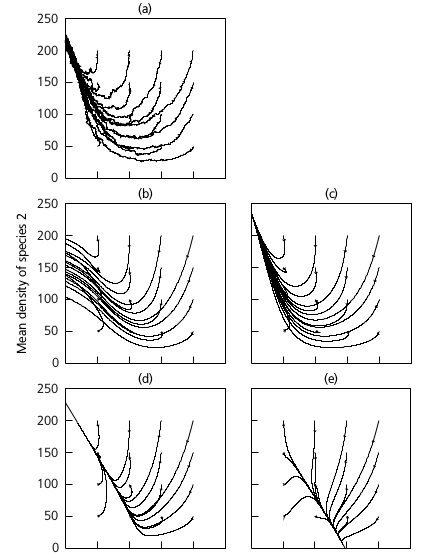
\includegraphics[width=.95\linewidth]{1234.png}
		\caption{Фазовый портрет в пространстве $[N_1; N_2]$: (a) --- для компьютерных симуляций; (b) -- (e) соответствуют решениям динамики по методы Рунге-Кутты для замыканий (1) -- (4) соответственно}
		\label{fig:comp1:1}
	\end{subfigure}% 
	\begin{subfigure}{.5\textwidth}
		\centering
		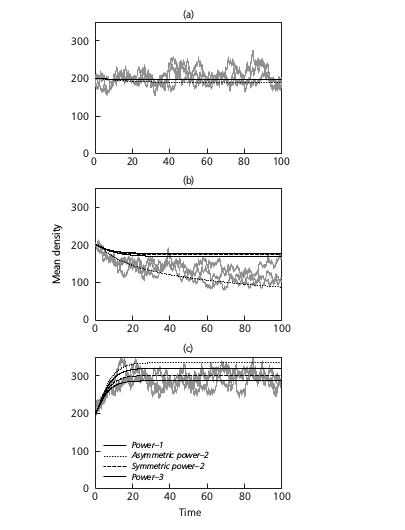
\includegraphics[width=.95\linewidth]{12345.jpg}
		\caption{Динамика первого момента $N(t)$ в случае одновидовой модели в сравнении с нескольким усредненными запусками симуляций} 
		\label{fig:comp1:2}
	\end{subfigure}
	\caption{Сравнение работы кандидатов в замыкания (1) -- (4) для одновидовых и двувидовых симуляций}
	\label{fig:comp1}
\end{figure*}

В то же время в \cite{murlaw} было предложено и исследовано параметрическое семейство замыканий:
\begin{multline}\label{eq:closure}
T_{ijk}(\xi,\xi')	=	\frac{\alpha}{2}\left(\frac{C_{ij}(\xi)C_{ik}(\xi')}{N_{i}}+\frac{C_{ij}(\xi)C_{jk}(\xi'-\xi)}{N_{j}}+\right.\\ 
\left.+\frac{C_{ik}(\xi')C_{jk}(\xi'-\xi)}{N_{k}}-1\right)+(1-\alpha)\frac{C_{ij}(\xi)C_{ik}(\xi')}{N_{i}},
\end{multline}
которое является линейной комбинацией замыканий (2) и (3). 
\begin{figure*}[ht]
	\centering
		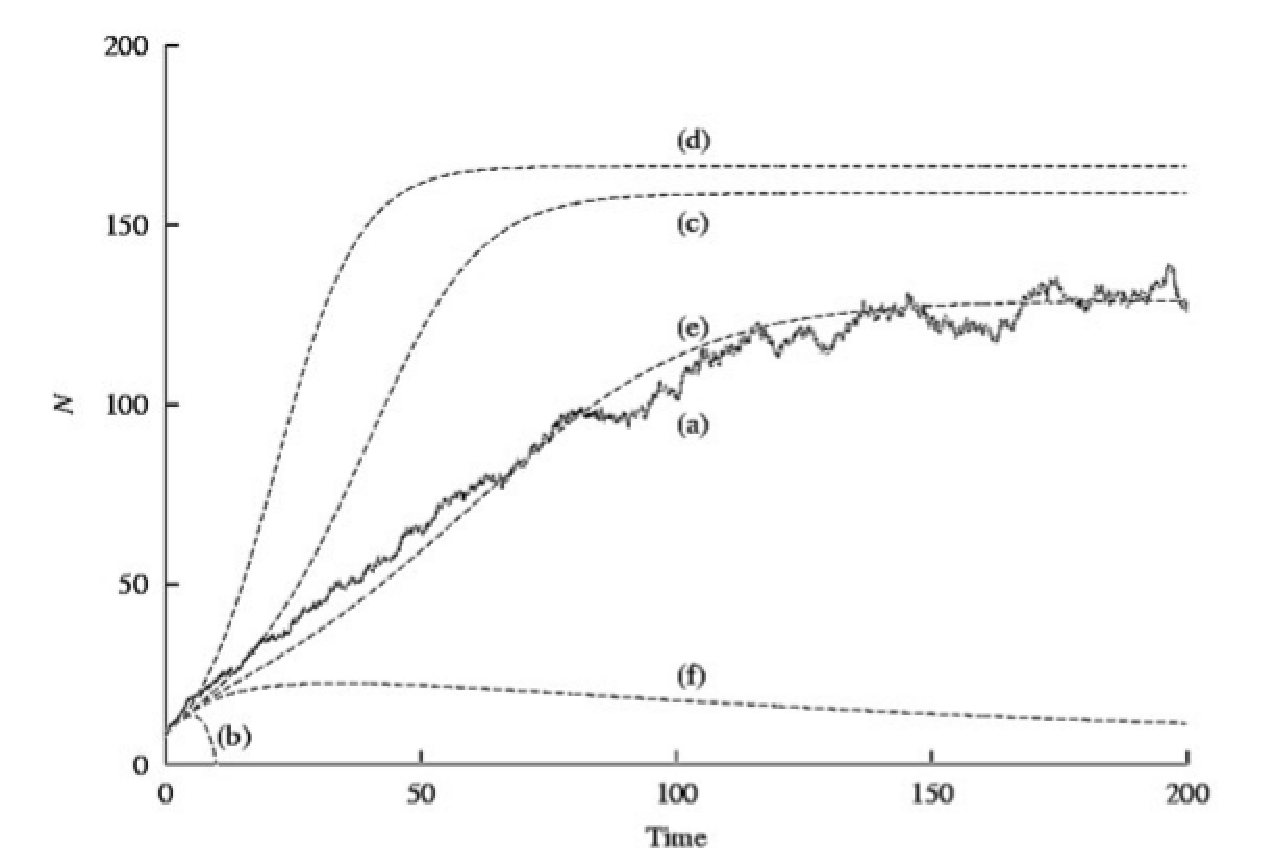
\includegraphics[width=.75\linewidth]{closures.eps}
		\caption{Сравнение работы различных представителей параметрического семейства замыканий с компьютерными симуляциями (a): (b) $\alpha = 1$; (c) $\alpha =0$; (d) $\alpha=1/4$; (e) $\alpha=2/5$}
	\label{fig:comp2}
\end{figure*}

Согласно результатам проверки на корректность различных представителей семейства предложенного замыкания в случае одновидовой системы, представленным на рис. \ref{fig:comp2}, наиболее подходящее под симуляции замыкание достигается при $\alpha = \frac{2}{5} $. Данное замыкание структурно достаточно близко к предложенной в \cite{as2} регуляризации, что приводит к совместной системе интегро-дифференциальных уравнений, в то время как предложенное замыкание работает более корректно; при всем этом стоит отдельно отметить, что используемое замыкание необязательно является наиболее подходящим и задача о поиске наиболее оптимального замыкания, не ограничиваясь выбранным семейством, является в известной мере одной из самых актуальных.
  \chapter{Постановка задачи}

После введение модели стационарных сообществ Ульфа Дикмана сформулируем условие поставленной перед нами задачи:


\textbf{Задача.} Найти стационарную точку системы:
\begin{equation*}
\forall i,j=1,2:\qquad\begin{cases}
\frac{dN_{i}(t)}{dt}=0,\\
\;\;\;\vdots\\
\frac{dC_{ij}(\xi,t)}{dt}=0
\end{cases}
\end{equation*}
при условии, что 
\begin{itemize}
	\item $ i,j=1,\;2 \forall i,j $ функция $ C_{ij}(\xi,t) $ радиально-симметрична; 
	\item ядра рождаемости $ m_{i}(\xi) $ и конкуренции $ w_{ij}(\xi) $ распределены нормально с нулевым математическим ожиданием;
	\item для разрешения иерархии зависимостей использовать замыкание \ref{eq:closure} c $\alpha=2/5$ \begin{multline*}
T_{ijk}(\xi,\xi')=\frac{1}{5}\left(\frac{C_{ij}(\xi)C_{ik}(\xi')}{N_{i}}+\frac{C_{ij}(\xi)C_{jk}(\xi'-\xi)}{N_{j}}+\right.\\
\left.+\frac{C_{ik}(\xi')C_{jk}(\xi'-\xi)}{N_{k}}-1\right)+\frac{3}{5}\cdot\frac{C_{ij}(\xi)C_{ik}(\xi')}{N_{i}};
\end{multline*}
\end{itemize}
С учетом того, что динамика системы описывается уравнениями:
\begin{align*}
\frac{d}{dt}N_{i}=(b_{i}-d_{i})N_{i}-\sum_{j}\int_{\mathbb{R}^{n}}w_{ij}(\xi)C_{ij}(\xi)d\xi \\
\frac{d}{dt}C_{ij}(\xi)	=	\delta_{ij}m_{i}(-\xi)N_{i}+\int_{\mathbb{\mathbb{R}}^{n}}m_{i}(\xi')C_{ij}(\xi+\xi')d\xi'-d_{i}C_{ij}(\xi)-\\
-\sum_{k}\int_{\mathbb{\mathbb{R}}^{n}}w_{ik}(\xi')T_{ijk}(\xi,\xi')d\xi-w_{ij}(\xi)C_{ij}(\xi)+\langle i,j,\xi\to j,i,-\xi\rangle
\end{align*}

\section{Результирующая система}
Прежде чем обратиться к выведению получающейся системы, введем несколько дополнительных обозначений и договоренностей:
\begin{itemize}
	\item поскольку изучается стационарное состояние системы, будем опускать зависимость функций-пространственных моментов от времени для удобства записи;
	
	\item для приведения системы уравнений к виду, удобному для решения численным методом переобозначим искомые функции следующим образом, нормируя и центрируя на пределы:
	\begin{equation*}
	C_{ij}(\xi)=\frac{C_{ij}(\xi)}{N_iN_j},
	\qquad
	 T_{ijk}(\xi, \xi')=\frac{T_{ijk}(\xi, \xi')}{N_iN_jN_k} 
	\end{equation*}
	\begin{equation*}
	D_{ij}(\xi)=C_{ij}(\xi)-1
	\end{equation*}
	Таким образом, $\lim\limits_{\xi \to \infty} C_{ij}(\xi)=1$, $\lim\limits_{\xi \to \infty} D_{ij}(\xi)=0$;
	\item свертку двух функций будем обозначать $\int_{\mathbb{R}^n} f(y)g(x+y)dx=[f*g](x)$;
	\item введем упрощающее обозначение $y_{ij}=\int\limits_{\mathbb{R}^n} w_{ij}(\xi)C_{ij}(\xi)d\xi$ --- агрегированный конкурентный фон с учетом пространственной структуры.
\end{itemize}

Пользуясь радиальной симметричностью функций-ядер и тем фактом, что $C_{21}(\xi)=C_{12}(-\xi)$, получаем:
\begin{equation*}
[m_{2}*C_{21}](-\xi)=\int_{-\infty}^{+\infty}m_{2}(\xi')C_{21}(\xi'-\xi)d\xi'=\int_{-\infty}^{+\infty}m_{2}(\xi')C_{12}(\xi-\xi')=[m_{2}*C_{12}](\xi)
\end{equation*}
Запишем уравнение на $C_{12}(\xi)$, раскрывая знаки суммирования:
\begin{multline*}
\frac{d}{dt}C_{12}(\xi)=[m_{1}*C_{12}](\xi)-d_{1}C_{12}(\xi)-\\
-\left(d{}_{11}^{'}\int w_{11}(\xi')T_{121}(\xi,\xi')d\xi'+d'_{12}\int w_{22}(\xi')T_{122}(\xi,\xi')d\xi'\right)-\\
-w_{12}(\xi)C_{12}(\xi)+[m_{2}*C_{21}](-\xi)-d_{2}C_{21}(-\xi)-\\
-\left(d_{21}^{'}\int w_{21}(\xi')T_{211}(-\xi,\xi')d\xi'+d'_{22}\int w_{22}(\xi')T_{212}(-\xi,\xi')d\xi'\right)-w_{21}(-\xi)C_{21}(-\xi)
\end{multline*}
Применим полученное отношение на свертки функций с разным знаком:
\begin{multline*}
\frac{d}{dt}C_{12}(\xi)=-\left(\int w_{21}(\xi')T_{211}(-\xi,\xi')d\xi'+\int w_{22}(\xi')T_{212}(-\xi,\xi')d\xi'+\right.\\
\left.+\int w_{11}(\xi')T_{121}(\xi,\xi')d\xi'+\int w_{12}(\xi')T_{122}(\xi,\xi')d\xi'\right) + \\
+[(m_{1}+m_{2})*C_{12}](\xi)-(d_{1}+d_{2}+w_{12}(\xi)+w_{21}(\xi))C_{12}(\xi)
\end{multline*}
В нормированном виде 
\begin{multline*}
\frac{d}{dt}C_{12}(\xi)=[(m_{1}+m_{2})*C_{12}](\xi)-(d_{1}+d_{2}+w_{12}(\xi)+w_{21}(\xi))C_{12}(\xi)-\\
-(N_{1}\int w_{21}(\xi')T_{211}(-\xi,\xi')d\xi'+N_{2}\int w_{22}(\xi')T_{212}(-\xi,\xi')d\xi'+\\
+N_{1}\int w_{11}(\xi')T_{121}(\xi,\xi')d\xi'+N_{2}\int w_{12}(\xi')T_{122}(\xi,\xi')d\xi')
\end{multline*}
Необходимо подставить нормированное замыкание, которые принимает слеюущий вид:
\begin{multline*}
T_{ijk}(\xi,\xi')=\frac{\alpha}{2}(C_{ij}(\xi)C_{ik}(\xi')+C_{ij}(\xi)C_{jk}(\xi-\xi')+C_{ik}(\xi')C_{jk}(\xi-\xi')-1)+(1-\alpha)C_{ij}(\xi)C_{ik}(\xi')
\end{multline*}
В итоге получаем (для удобства чтения, в каждой строке сгруппированы слагаемые с одним и тем же параметрическим множителем, который указан в правом нижем углу):
\begin{align*}
N_{1}\int w_{21}(\xi')T_{211}(-\xi,\xi')d\xi'+N_{2}\int w_{22}(\xi')T_{212}(-\xi,\xi')d\xi'+		\\
+N_{1}\int w_{11}(\xi')T_{121}(\xi,\xi')d\xi'+N_{2}\int w_{12}(\xi')T_{122}(\xi,\xi')d\xi'	|_{C(\xi)C(\xi')}=	\\
=N_{1}C_{12}y_{21}+N_{2}C_{12}y_{22}+N_{1}C_{12}y_{11}+N_{2}C_{12}y_{12} &&		\times(1-\frac{\alpha}{2})
\end{align*}
где подстановка $T_{ijk}(\xi, \xi')=C_{ij}(\xi)C_{ik}(\xi')$ обозначена как 	$|_{C(\xi)C(\xi')}$.

Воспользуемся уравнениями на первые моменты:
\begin{equation*}
\begin{cases}
N_{1}y_{11}+N_{2}y_{12}=b_{1}-d_{1}\\
N_{1}y_{21}+N_{2}y_{22}=b_{2}-d_{2}
\end{cases}
\end{equation*}
Получаем:
\begin{align*}
N_{1}\int w_{21}(\xi')T_{211}(-\xi,\xi')d\xi'+N_{2}\int w_{22}(\xi')T_{212}(-\xi,\xi')d\xi'+		\\
+N_{1}\int w_{11}(\xi')T_{121}(\xi,\xi')d\xi'+N_{2}\int w_{12}(\xi')T_{122}(\xi,\xi')d\xi'	|_{C(\xi)C(\xi')}=	\\
=(b_{1}+b_{2}-d_{1}-d_{2})C_{12}(\xi)	=	\\
=(b_{1}+b_{2}-d_{1}-d_{2})D_{12}(\xi)+(b_{1}+b_{2}-d_{1}-d_{2}) &&		\times(1-\frac{\alpha}{2})
\end{align*}
По линейности интеграла, подставим замыкание и раскроем получающееся выражение:
\begin{align*}
N_{1}\int w_{11}(\xi')T_{121}(\xi,\xi')d\xi'+N_{2}\int w_{12}(\xi')T_{122}(\xi,\xi')d\xi'+		\\
+N_{1}\int w_{21}(\xi')T_{211}(-\xi,\xi')d\xi'+N_{2}\int w_{22}(\xi')T_{212}(-\xi,\xi')d\xi'|_{C(\xi)C(\xi-\xi')}	=	\\
=N_{1}C_{12}[w_{11}*C_{21}]+N_{2}C_{12}[w_{12}*C_{22}]+N_{1}C_{12}[w_{21}*C_{11}]+N_{2}C_{12}[w_{22}*C_{12}]	= \\	
=(D_{12}+1)(N_{1}[w_{11}*D_{21}]+N_{2}[w_{12}*D_{22}]+N_{1}[w_{21}*D_{11}]+N_{2}[w_{22}*D_{12}]+ \\		
+N_{2}d'_{22}+N_{1}d'_{21}+N_{2}d_{22}^{'}+N_{1}d{}_{11}^{'})		&& \times\frac{\alpha}{2}
\end{align*}
Аналогично поступим для оставшегося блока, также воспользовавшись уравнениями для динамики первых моментов:
\begin{align*}
N_{1}\int w_{21}(\xi')T_{211}(-\xi,\xi')d\xi'+N_{2}\int w_{22}(\xi')T_{212}(-\xi,\xi')d\xi'		\\
+N_{1}\int w_{11}(\xi')T_{121}(\xi,\xi')d\xi'+N_{2}\int w_{12}(\xi')T_{122}(\xi,\xi')d\xi'|_{C(\xi')C(\xi-\xi')}	=	\\
=N_{1}[w_{21}C_{12}*C_{11}]+N_{2}[w_{22}C_{22}*C_{12}]+N_{1}[w_{11}C_{11}*C_{12}]+N_{2}[w_{12}C_{12}*C_{22}]	=	\\
=\{N_{1}[(w_{12}D_{12}+w_{12})*(D_{22}+1)]\}	=	\\
=N_{1}[w_{21}D_{12}*D_{11}]+N_{1}[w_{21}*D_{11}]+N_{1}y_{21}	+	\\
+N_{2}[w_{12}D_{12}*D_{22}]+N_{2}[w_{12}*D_{22}]+N_{2}y_{12}	+	\\
+N_{1}[w_{11}D_{11}*D_{12}]+N_{1}[w_{11}*D_{12}]+N_{1}y_{11}	+	\\
+N_{2}[w_{22}D_{22}*D_{12}]+N_{2}[w_{22}*D_{12}]+N_{2}y_{22}	=	\\
=N_{1}[w_{21}*D_{11}]+N_{2}[w_{22}*D_{12}]+N_{1}[w_{11}*D_{12}]+N_{2}[w_{12}*D_{22}]	+	\\
+N_{1}[w_{21}D_{12}*D_{11}]+N_{2}[w_{22}D_{22}*D_{12}]+N_{1}[w_{11}D_{11}*D_{12}]+N_{2}[w_{12}D_{12}*D_{22}]	+	\\
+N_{1}d'_{21}+N_{2}d'_{22}+N_{1}d'_{11}+N_{2}d'_{12}	+	\\
+b_{1}+b_{2}-d_{1}-d_{2}	&&	\times\frac{\alpha}{2}
\end{align*}
Проссумируем три получившихся блока:
\begin{align*}
((1-\frac{\alpha}{2})(b_{1}+b_{2})+\frac{\alpha}{2}(d_{1}+d_{2})+w_{12}+w_{21})D_{12}=[(m_{1}+m_{2})*D_{12}]-w_{12}-w_{21}		\\
-\frac{\alpha}{2}(D_{12}(N_{1}[w_{11}*D_{21}]+N_{2}[w_{12}*D_{22}]+N_{1}[w_{21}*D_{11}]+		\\
+N_{1}[w_{21}D_{12}*D_{11}]+N_{2}[w_{22}D_{22}*D_{12}]+N_{1}[w_{11}D_{11}*D_{12}]+N_{2}[w_{12}D_{12}*D_{22}]) + \\
+2N_{1}[w_{11}*D_{21}]+2N_{2}[w_{12}*D_{22}]+2N_{1}[w_{21}*D_{11}]+2N_{2}[w_{22}*D_{12}]+	\\			
N_{2}[w_{22}*D_{12}]+N_{2}d'_{12}+N_{1}d'_{21}+N_{2}d_{22}^{'}+N_{1}d{}_{11}^{'})
\end{align*}
И приведем к итоговому виду:
\begin{align*}
((1-\frac{\alpha}{2})(b_{1}+b_{2})+\frac{\alpha}{2}(d_{1}+d_{2}+d'_{11}N_{1}+d'_{12}N_{2}+d'_{21}N_{1}+d'_{22}N_{2})+w_{12}+w_{21})D_{12}=	\\
[(m_{1}+m_{2})*D_{12}]-w_{12}-w_{21}-\\
-\frac{\alpha}{2}N_{1}((D_{12}+2)([w_{11}*D_{12}]+[w_{21}*D_{11}])+[w_{21}D_{12}*D_{11}]+[w_{11}D_{11}*D_{12}])-\\		
-\frac{\alpha}{2}N_{2}((D_{12}+2)([w_{12}*D_{22}]+[w_{22}*D_{12}])+[w_{22}D_{22}*D_{12}]+[w_{12}D_{12}*D_{22}])		
\end{align*}
Аналогичным образом преобразуем два оставшихся уравнения:
\begin{align*}
((1-\frac{\alpha}{2})b_{1}+\frac{\alpha}{2}(d_{1}+N_{1}d'_{11}+N_{2}d'_{12})+w_{11})D_{11}=\frac{m_{1}}{N_{1}}+\left[m_{1}*D_{11}\right]-w_{11}-\\
-\frac{\alpha}{2}N_{1}((D_{11}+2)[w_{11}*D_{11}]+[w_{11}D_{11}*D_{11}])-\\
-\frac{\alpha}{2}N_{2}((D_{11}+2)[w_{12}*D_{12}]+[w_{12}D_{12}*D_{12}])
\\
((1-\frac{\alpha}{2})b_{2}+\frac{\alpha}{2}(d_{2}+N_{1}d'_{21}+N_{2}d'_{22})+w_{22})D_{22}=\frac{m_{2}}{N_{2}}+\left[m_{2}*D_{22}\right]-w_{22}-\\
-\frac{\alpha}{2}N_{2}((D_{22}+2)[w_{22}*D_{22}]+[w_{22}D_{22}*D_{22}])-\\
-\frac{\alpha}{2}N_{1}((D_{22}+2)[w_{21}*D_{12}]+[w_{21}D_{12}*D_{12}])
\end{align*}
И решим линейную систему на $ N_{1} $ и $ N_{2} $:
\begin{align*}
N_{1}=\frac{(b_{1}-d_{1})y_{22}-(b_{2}-d_{2})y_{12}}{y_{11}y_{22}-y_{12}y_{21}}
\\
N_{2}=\frac{(b_{2}-d_{2})y_{11}-(b_{1}-d_{1})y_{21}}{y_{11}y_{22}-y_{12}y_{21}}
\end{align*}
Получившаяся система из пяти нелинейных интегральных уравнений описывает стационарное положение рассматриваемой популяции в пространстве.
  \chapter{Численный метод в пространствах разной размерностей }

\section{Численный метод для решения системы}

Перепишем полученную систему в операторном виде для дальнейшей работы:
\begin{equation*}
\begin{cases}
	N_{1}=L_{1}(y_{11},y_{12},y_{21},y_{22})\\
	N_{2}=L_{2}(y_{11},y_{12},y_{21},y_{22})\\
	D_{11}=K_{11}(N_{1},N_{2},D_{11},D_{12})\\
	D_{12}=K_{12}(N_{1},N_{2},D_{11},D_{12},D_{22})\\
	D_{22}=K_{22}(N_{1},N_{2},D_{21},D_{22})
\end{cases}
\end{equation*}
где $L_i$ --- линейный интегральные операторы, включающие $ \int_{\mathbb{R}^n}w_{ij}(\xi)C_{ij}(\xi)d\xi$, а $K_{ij}$ --- интеральные операторы с нелинейностями вида $ \int_{\mathbb{R}^n}w_{ik}(\xi)D_{ik}(\xi)d\xi$, $D_{ik}(\xi)\cdot [w_{ik}*D_{ik}](\xi)$ и $[(w_{ik}\cdot D_{ik})*D_{ik}](\xi)$. 

Дискретизация полученных уравнений приведет к системе алгебраических уравнений второго порядка; для решения этой системы применим \textit{метод рядов Неймана (метод последовательных приближений)}, который сойдется при условии сжатия по норме во всех итеративных точках. 

Опишем принцип работы данного метода. Пусть дано уравнение вида \begin{equation*}
\vec{f}=\vec{g}+K\vec{f},
\end{equation*}
где $K$ --- некоторый оператор, $\vec{g}$ --- известная функция, а $\vec{f}$ --- искомая.

\textbf{Теорема 1.} Ряд 
\begin{equation*}
	\vec{g}+K\vec{g}+K^2\vec{g}+\ldots+K^n\vec{g}+\ldots
\end{equation*}
	в случае своей сходимости сходится к решению уравнения выше.\\
\textit{Доказательство. }\ Действительно, $\vec{g}+K\vec{f}=\vec{g}+K(\vec{g}+K\vec{g}+K^2\vec{g}+\ldots+K^n\vec{g}+\ldots)=\vec{g}+K\vec{g}+K^2\vec{g}+\ldots+K^n\vec{g}+\ldots=\vec{f}$, что и требовалось доказать.

\textbf{Теорема 2.} Если оператор $K$ --- сжимающий, т.е.
\begin{equation*}
	\exists \alpha,\;0<\alpha<1:\;\forall \vec{x}, \vec{y} \Rightarrow \rho(K\vec{x}, K\vec{y})<\alpha\cdot\rho(\vec{x}, \vec{y}),
\end{equation*}
	то ряд  $\vec{g}+K\vec{g}+K^2\vec{g}+\ldots+K^n\vec{g}+\ldots$ сходится.\\
\textit{Доказательство.} По теореме Банаха у сжимающего отображения в полном метрическом пространстве существует неподвижная точка, при том только одна. Значит, ряд сходится.

Далее приведем алгоритм работы численного метода:

\begin{enumerate}
	\item Инициализируем процесс $N_1=N_2=0$, $D_{11}=D_{12}=D_{22}=0$; формально говоря, в большинстве запусков в рамках данной работы инициализация будет проводится не нулевыми значениями, а известной стационарной точкой для близких параметров системы;
	\item Пересчитаем последовательно $D_{12}=K_{12}(N_1, N_2, D_{11}, D_{12}, D_{21})$;
	\item Зная новый $D_{12}$, пересчитаем:
	\begin{align*}
	N_1=L_1(y_{11}, y_{12}, y_{21}, y_{22}) \\
	N_2=L_2(y_{11}, y_{12}, y_{21}, y_{22})
	\end{align*}
	\item Пересчитаем
	\begin{align*}
	D_{11}=K_{11}(N_{1},N_{2},D_{11},D_{12})\\
	D_{22}=K_{22}(N_{1},N_{2},D_{21},D_{22})
	\end{align*}
	\item Итеративно повторим, пока суммарная относительная ошибка всех неизвестных величин не станет меньше выбранной величины; для дальнейших вычислений выбиралась метрика $\mathbb{L}_1$ для сравнения функциональных погрешностей и $\varepsilon=10^{-8}$.
\end{enumerate}

\section{Эвристики численного метода в случаях $ \mathbb{R}^2 $}

Далее обратимся к изучению двумерного случая. Наиболее сложным с вычислительной точки зрения вопросом является работа с двумерной сверткой. Для нее верно свойство преобразования Фурье: 
 \begin{equation*}
[f*g]_{\mathbb{R}^{2}}=\hat{F}[F[f]\cdot F[g]],
\end{equation*}
где $\hat{F}[h]$ --- обратное преобразование Фурье. После дискретизации на квадратной сетке размера $ K\times K $ прямое и обратное преобразования выглядят следующим образом:
\begin{equation*}
 G_{uv}=\frac{1}{K^{2}}\sum\limits _{n=1}^{K-1}\sum\limits _{m=1}^{K-1}x_{mn}e^{-\frac{2i\pi}{K}(mu+nv)},
\end{equation*}
\begin{equation*}
 x_{nm}=\sum\limits _{n=1}^{K-1}\sum\limits _{m=1}^{K-1}G_{uv}e^{\frac{2i\pi}{K}(mu+nv)}.
\end{equation*}
 Эти преобразования могут быть ускорены за счет применения одномерного быстрого преобразования Фурье: 
\begin{equation*}
G_{uv}=\frac{1}{K}\sum\limits _{n=1}^{K-1}\left[\frac{1}{K}\sum\limits _{m=1}^{K-1}x_{mn}e^{-\frac{2i\pi nv}{K}}\right]e^{-\frac{2i\pi mu}{K}}, 
\end{equation*}
что дает алгоритмическую сложность $ O(K^{3}\log(K)) $, поскольку необходимо вычислить быстрое преобразование Фурье ($ K\log(K) $) в каждом узле сетки \cite{Press1996}. Данную асимптотику можно улучшить, применив преобразование Ханкеля \cite{Baddour:09}. 

Перейдем в преобразовании Фурье к полярным координатам: 
\begin{equation*}
 F[f](\omega_{x},\omega_{y})=\int\limits _{-\infty}^{+\infty}\int\limits _{-\infty}^{+\infty}f(x,y)e^{-i(\omega_{x}x+\omega_{y}y)}dxdxy=\int\limits _{0}^{+\infty}\int\limits _{-\pi}^{\pi}f(r,\theta)e^{-ir\rho\cos(\psi-\theta)}rdrd\theta.
\end{equation*}
Пользуясь тем, что исследуемые функции радиально-симметричны, получаем соотношение 
\begin{equation*}
F[f](\rho,\psi)=\int\limits _{0}^{+\infty}rf(r)dr\int\limits _{-\pi}^{\pi}e^{-ir\rho\cos(\psi-\theta)}d\theta=2\pi\int\limits _{0}^{+\infty}rf(r)J_{0}(r\rho)dr, 
\end{equation*}
которое известно как \textbf{{преобразование Ханкеля 0-го порядка}}, где $ J_{0}(x)=\frac{1}{2\pi}\int\limits _{-\pi}^{\pi}e^{-ix\cos\tau}d\tau $ --- \textit{функция Бесселя нулевого порядка}. Если же теперь дополнительно сделать экспоненциальную замену переменных $ r=r_{0}e^{x} $, $ \rho=\rho_{0}e^{y} $, 
\begin{equation*}
H_{0}[f](\rho)=\int_{0}^{+\infty}rf(r)J_{o}(\rho r)dr=\frac{1}{e^{y/4}}[(f(e^{x/4})\cdot e^{x/4})*J_{0}(e^{x/4})](y)|_{x=\ln r,\;y=\ln\rho}.
\end{equation*}
то вместо преобразования Фурье получим свертку двух функций, алгоритмическая сложность которой $ O(K\cdot\log(K)) $, т.е. было произведено ускорение в $ K^{2} $ раз.

\section{Эвристики численного метода в случаях $ \mathbb{R}^3 $}

Аналогичным образом проведем рассуждение в случае трехмерной свертки. Для нее верно свойство преобразования Фурье: 
\begin{equation*}
[f*g]_{\mathbb{R}^{3}}=\hat{F}[F[f]\cdot F[g]],
\end{equation*}
где $\hat{F}[h]$ --- обратное преобразование Фурье. Пользуясь соображениями выше, легко понять, что ее вычислительная сложность есть не что иное, как быстрое преобразование Фурье, запущенное в каждой точке пространства, т.е. $ O(K^{3}\cdot K\log K)=O(K\cdot\log K) $. Улучшим вычислительную сложность нашего метода за счет перехода в класс радиально симметричных функций, как и ранее. Для этого сделаем дополнительное построение: вспомним задачу Лапласса с граничным условием на шаре:
\begin{equation*}
\begin{cases}
	\Delta u=0\\
	0<\rho<a,\;0<\theta<\pi,\;0<\phi<2\pi\\
	u(a,\theta,\phi)=f_{0}(\theta,\phi)\equiv0
\end{cases}
\end{equation*}
Строго говоря, мы необязаны привязывать наши рассуждения к конкретному виду начальных условий, поэтому для удобства положим, что задача дана с условиями Дирихле, как приведено выше. Перепишем:
\begin{equation*}
\begin{cases}
\frac{1}{r^2} \frac{\partial}{\partial r}\left(r^2 \frac{\partial u}{\partial r}\right) + \frac{1}{r^2 \sin \theta} \frac{\partial}{\partial \theta }\left(\sin \theta \frac{\partial u}{\partial \theta }\right)+\frac{1}{r^2 \sin^2 \theta } \frac{\partial^2 u}{\partial \phi^2}=0\\
0<\rho<a,\;0<\theta<\pi,\;0<\phi<2\pi\\
u(a,\theta,\phi)=f_{0}(\theta,\phi)
\end{cases}
\end{equation*}
Положим $u=R(r)Y(\theta, \phi)$. Тогда:
\begin{equation*}
Y \frac{d}{dr}(r^2 R')+R\left[ \frac{1}{ \sin \theta} \frac{\partial}{\partial \theta }\left(\sin \theta \frac{\partial Y}{\partial \theta }\right)+\frac{1}{\sin^2 \theta } \frac{\partial^2 Y}{\partial \phi^2}\right]=0
\end{equation*}
Откуда получаем по классической схеме постоянной разделения:
\begin{align*}
r^2R''+2rR'-\lambda R =0 \\
\frac{1}{ \sin \theta} \frac{\partial}{\partial \theta }\left(\sin \theta \frac{\partial Y}{\partial \theta }\right)+\frac{1}{\sin^2 \theta } \frac{\partial^2 Y}{\partial \phi^2}+\lambda Y = 0
\end{align*}
Так же, как и выше, для второго уравнения разделим переменные $Y(\theta, \phi)=F(\theta)G(\phi)$:
\begin{equation*}
G\frac{1}{ \sin \theta} \frac{\partial}{\partial \theta }\left( \theta F'\right)+\frac{1}{\sin^2 \theta }FG''+\lambda FG = 0
\end{equation*}
Откуда аналогичным разделением переменных получаем:
\begin{align*}
G''+\mu G = 0 \\
\frac{1}{ \sin \theta} \frac{\partial}{\partial \theta }\left( \theta F'\right)+\left(\lambda - \frac{\mu}{\sin^2\theta}\right)F=0
\end{align*}
Из первого уравнения, зная собственные числа оператора второй производной, получаем, что $\mu=n^2$. Во втором уравнении сделаем, замену $t=\cos \theta$:
\begin{align*}
G'=G'_t(-\sin\theta) \\
G''=G''_{tt}\sin^2\theta -G'_t\cos\theta
\end{align*}
Тогда мы получаем классическое уравнение:
\begin{equation*}
(1-t^2)G''_{tt}-2tG'_t+\left(\lambda - \frac{n^2}{1-t^2}\right)G=0
\end{equation*}
где собственный базис есть $ P_{n}^{k}(t) $ --- \textit{присоединенные полиномы Лежандра}, известные своей ортогональностью в $ L_{2} $: \begin{equation*}
P_{n}^{k}(t)=\frac{(-1)^{n}}{n!2^{n}}(1-t^{2})^{k/2}\frac{d^{n+k}}{dt^{n+k}}[(1-t^{2})^{n}],
\end{equation*}
т.е. 
\begin{equation*}
G(t)=\sum\limits_0^\infty A_n \frac{(-1)^{n}}{n!2^{n}}(1-t^{2})^{k/2}\frac{d^{n+k}}{dt^{n+k}}[(1-t^{2})^{n}]
\end{equation*}
Возвращаясь к неизвестной функции и меняя порядок суммирования, чтобы привести к виду метода Фурье $ u(\rho,\theta,\phi)=\sum\limits _{n=0}^{+\infty}\sum\limits _{k=-n}^{n}R_{n}^{k}(\rho)Y_{n}^{k}(\theta,\phi) $ для решения дифференциальных уравнений в частных производных, получаем: \begin{equation*}
Y_{n}^{k}(\theta,\phi)=\sqrt{\frac{(2n+1)(n-k)!}{4\pi(n+k)!}}P_{n}^{k}(\cos\phi)e^{ik\theta},
\end{equation*}
Воспользуемся разложением ядра Фурье через $ Y_{n}^{k} $ \cite{Baddour:10}: \begin{equation*}
e^{i(\vec{w},\vec{r})}=4\pi\sum\limits _{n=0}^{+\infty}\sum\limits _{k=-n}^{n}(-1)^{n}\sqrt{\frac{\pi}{2r\rho}}J_{n+1/2}(\rho r)\overline{Y_{n}^{k}(\phi,\psi)}Y_{n}^{k}(\theta,\eta)
\end{equation*}
Подставляя полученное выражение в теорему о свертке:
\begin{multline*}
[f***g]=F^{-1}[ F[f]\cdot F[g] ]= \int\limits_{\mathbb{R}^3} \left[ \left( \int\limits_{\mathbb{R}^3} f(r) e^{i (\vec{w}, \vec{r})} r^2 \sin \phi dr d\phi \right) \cdot \right. \\
\left. \cdot \left( \int\limits_{\mathbb{R}^3} g(r) e^{i (\vec{w}, \vec{r})} r^2 \sin \phi dr d\phi \right) \right] e^{-i (\vec{w}, \vec{r})} \rho^2 \sin \theta d\rho d\theta d\eta
\end{multline*}
и меняя порядок суммирования с учетом ортогональности полиномов Лежандра, получаем ненулевым только первое слагаемое с обычной полярной заменой координат: 
\begin{multline*}
[f***g]=F^{-1}[ F[f]\cdot F[g] ]=\\
= \int\limits_{\mathbb{R}^3} \left[  \int\limits_{\mathbb{R}^3 \times \mathbb{R}^3} f(r) 4\pi\sum\limits _{n=0}^{+\infty}\sum\limits _{k=-n}^{n}(-1)^{n}\sqrt{\frac{\pi}{2r\rho}}J_{n+1/2}(\rho r)\overline{Y_{n}^{k}(\phi,\psi)}Y_{n}^{k}(\theta,\eta) r^2 \sin \phi dr d\phi \right. \cdot \\ \cdot \left. g(r) 4\pi\sum\limits _{n=0}^{+\infty}\sum\limits _{k=-n}^{n}(-1)^{n}\sqrt{\frac{\pi}{2r\rho}}J_{n+1/2}(\rho r)\overline{Y_{n}^{k}(\phi,\psi)}Y_{n}^{k}(\theta,\eta)e^{i (\vec{w}, \vec{r})} r^2 \sin \phi dr d\phi \right] e^{-i (\vec{w}, \vec{r})} \rho^2 \sin \theta d\rho d\theta d\eta
\end{multline*}
Что в итоге сворачивается к следующей формуле, позволяющей также, как и в двумеоном случае, свести вычислительную сложность к сложности одномерной задачи:
\begin{equation*}
[f***g](\vec{r})=4\pi[(r\cdot f)*g](r)
\end{equation*}
  \chapter{Continued captions}
\label{chap:ContCaptions}

Here are some funky floats using ``continued captions'', i.e. for a semantically
collected group of float contents which are too numerous to fit into a single
float, such as the pretty circles in the following figure:

\newcommand{\circleimg}[1]{%
\begin{tikzpicture}
  \draw[color=black,fill=#1,thick] (1,0) circle (1.5cm);
\end{tikzpicture}%
}

\begin{figure}[hb]
  \subfloat[][Example 1a]{\label{fig:cc1a}\circleimg{red!80}}\quad
  \subfloat[][Example 1b]{\label{fig:cc1b}\circleimg{green!70!yellow}}\quad
  \subfloat[][Example 1c]{\label{fig:cc1c}\circleimg{blue!80}}\quad
  \subfloat[][Example 1d]{\label{fig:cc1d}\circleimg{orange!80!yellow}}
  \caption{Demonstration of \texttt{subfig} continued captions.}
  \label{fig:cc1}
\end{figure}

\begin{figure}[p]
  \ContinuedFloat
  \subfloat[][Example 1e]{\label{fig:cc1e}\circleimg{violet}}\quad
  \subfloat[][Example 1f]{\label{fig:cc1f}\circleimg{cyan}}\quad
  \subfloat[][Example 1g]{\label{fig:cc1g}\circleimg{magenta}}\quad
  \subfloat[][Example 1h]{\label{fig:cc1h}\circleimg{yellow}}
  \caption[]{Demonstration of \texttt{subfig} continued captions (continued).}
\end{figure}

\noindent
This mechanism means that the same float label is used for both pages of
floats. Note that we can refer to %\FigureRef{fig:cc1} in general, or to
%\FigureRef{fig:cc1g} on \PageRef{fig:cc1g} in particular!

\noindent
Just for the hell of it, let's also refer to \SectionRef{sec:neutralmixing}.

\end{mainmatter}

\begin{backmatter}
    %\begin{colophon}
%  This thesis was made in \LaTeXe{} using the ``hepthesis'' class~\cite{hepthesis}.
%\end{colophon}

%% You're recommended to use the eprint-aware biblio styles which
%% can be obtained from e.g. www.arxiv.org. The file mythesis.bib
%% is derived from the source using the SPIRES Bibtex service.
%\bibliographystyle{h-physrev}
\bibliographystyle{abbrv}
\bibliography{mythesis}

%% I prefer to put these tables here rather than making the
%% front matter seemingly interminable. No-one cares, anyway!
\listoffigures
\listoftables

%% If you have time and interest to generate a (decent) index,
%% then you've clearly spent more time on the write-up than the 
%% research ;-)
%\printindex

\end{backmatter}

\end{document}
